The primary objective in machine learning (and therefore deep learning) is to perform well on new, unseen data.  The central challenge is finding the ideal balance between \textbf{overfitting} and \textbf{underfitting}.  In order to accomplish this balancing act, model performance is rated by its prediction on a test set and regulated to preserve the flexibility of a high-parameter network.

\subsection{Rating Model Performance}

%start with \cite{Goodfellow-et-al-2016} (ch 5)

During the build process, a model is faced with a training set and measured against a test set.  With the training set, the model engages its optimization techniques (i.e. gradient decent) in order to minimize a cost function (i.e. least squares).  The measure of error that is used to optimize parameters based on reducing its theoretic value is known as the \textit{training error}.  When model performance on new predictions is measured against the test set, the expected value of the error between predictions and actual test data is the \textit{test error} (commonly referred to as the \textit{generalization error}). \cite{Goodfellow-et-al-2016}

 When the model cannot obtain a sufficiently low training error, it is \textit{underfit}.  This happens when a linear model is applied to a non-linear set of observations, as shown in Figure \ref{capacityviz}.  Additional processing is enrolled to accommodate the model to the data contours, creating a model with a lower error; but attempting to fit the model too closely to the data creates a model with additional bias.  Often times, when a model is optimized toward a minimum training error, test error passes through a minimum rather than decreasing monotonically \cite{mackay1992bayesian}.  When the gap between the training error and test error is too great, the model is \textit{overfit}.
 %Figure \ref{capacityviz} displays a linear regression model under circumstances where it is underfit and where it is overfit.
 
 \begin{figure}[H]
    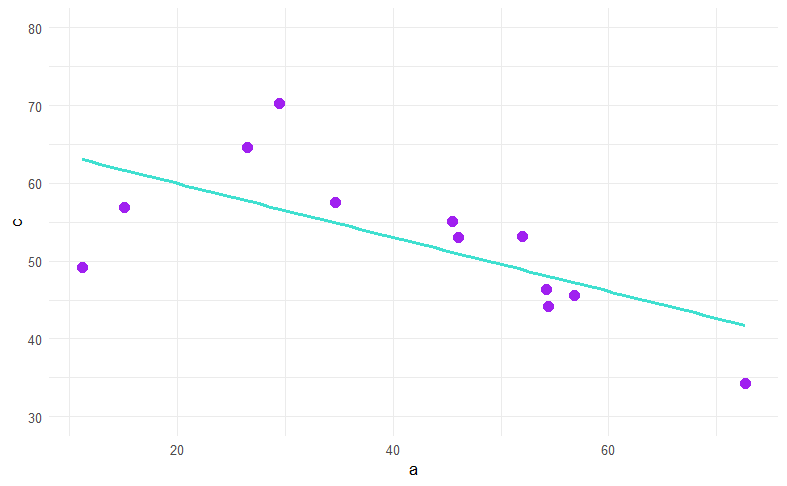
\includegraphics[width=0.5\linewidth]{Figures/underfit.png}
    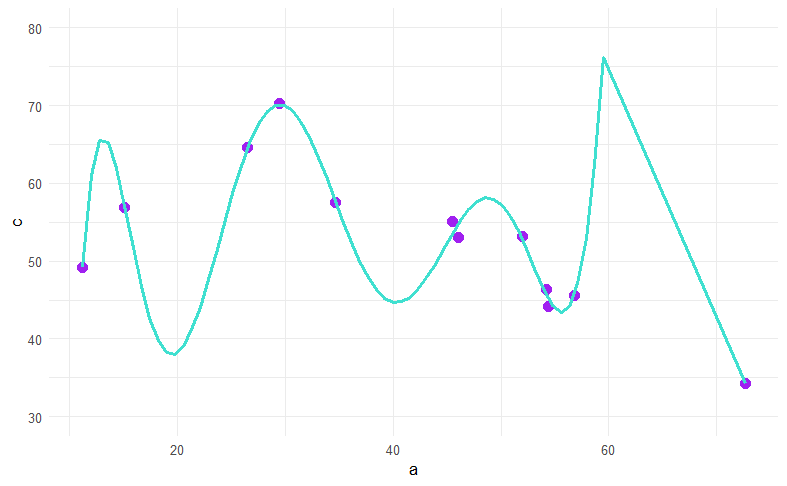
\includegraphics[width=0.5\linewidth]{Figures/overfit.png}
    \vspace{-20pt}
    \caption{\footnotesize{The regression model to the left has minimal capacity.  It underfits the data. The model to the right depicts an overfitting model.}}
    \label{capacityviz}
\end{figure}
 
 Somewhere between these extremes is the model's optimal \textit{capacity}.  Capacity is a model's ability to fit a wide variety of functions, and machine learning models perform best when their capacity is appropriate for the complexity of the task \cite{Goodfellow-et-al-2016}.  In linear regression, increasing the model's capacity would be to include polynomial terms or spline regression to shape the model beyond a straight line, as shown in Figure \ref{capacityviz}.  For neural networks, adding additional neurons or hidden layers increases model capacity.
 Because a neural network model has many more parameters to be estimated than its linear regression counterpart, it is much more susceptible to overfitting.  As capacity increases, so too does the amount of data needed for the network to be able to generalize \cite{baum1988size}.

%- \textbf{Generalization}

\subsection{Addressing Model Performance}

There is no one way to set the dials of a neural network.  Generally, they are established by trial and error, train/test split, or more sophisticated techniques as cross-validation to compare networks trained with different parameter values \cite{mackay1992practical}.  The class of techniques used to calibrate the model toward training data with a focus on generalizability for new data is known as \textbf{regularization}.  This is really any modification made to the learning process that aims to reduce test error (but not training error) \cite{Goodfellow-et-al-2016}.  This thesis covers three common techniques to regularize neural networks: \textit{Early stopping}, \textit{dropout}, and \textit{weight decay}.

\textit{Early stopping} is when the optimization algorithm is halted before the test error increases too much.  It is hoped that the algorithm stops at an optimal model capacity. To do this, as the model is being fit to the training data, its test error is simultaneously calculated. 
 Often, the algorithm stops when the test error reaches a minimum. \cite{doan2004generalization}

 \begin{figure}[H]
    \centering
    \vspace{-0pt}
    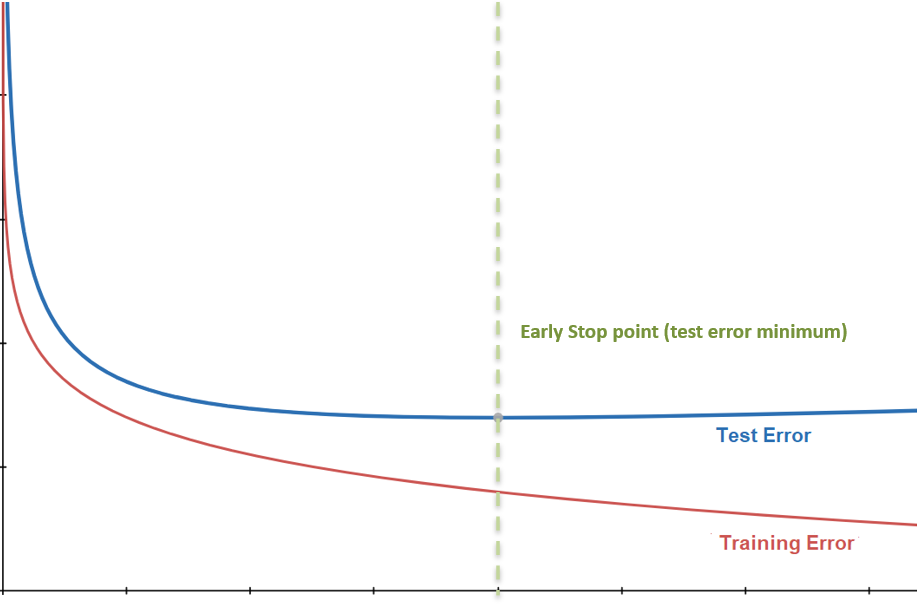
\includegraphics[width=0.5\linewidth]{Figures/early_stop.png}
    \caption{\footnotesize Often, as training error is reduced, test error passes through a minimum.  early stopping generally tells the optimization algorithm to stop when this is reached.}
    \label{earlystop}
\end{figure}

\textit{Dropout} refers to the technique of temporarily removing neurons (and all involved connections) at random  at each iteration of training.\cite{srivastava2014dropout}  For example, a dropout with control parameter $p_{drop} = .25$ means that at each cycle of training, a random 75\% of the network is used and a new 75\% is sampled for the next step. This simultaneously speeds up computation as well as prevents overfitting because it reduces the number of calculations at each step of the model building process.

\textit{Weight decay} is the neural network equivalent to shrinkage in machine learning.  For more information on shrinkage and regularization techniques in traditional machine learning, see (Goodfellow, 2016) \cite{Goodfellow-et-al-2016}.
Weight decay is when a  term is added to the optimizer to penalize weights in hopes to achieve a smoother fit \cite{mackay1992practical}.  The penalty term forces the weight coefficients to be small because the optimizer seeks to reduce the overall function.  To illustrate, suppose a network architecture $\mathcal{A}$ is defined for a model.  This architecture contains the specifications of the number of layers, neurons in each layer, activation functions, and available connections between layers.  The function mapping is defined as $\hat{y}(x_i;W,\mathcal{A})$, which outputs an estimated value for each input $x_i$ from the given architecture $\mathcal{A}$ and set of weights $W$.  If the gradient descent algorithm is used to find optimal parameter values based on minimizing the following loss function $E_D$:
$$
E_D(D|W,\mathcal{A}) = \sum_i [\hat{y}(x_i;W,\mathcal{A}) - y_i]^2
$$

%commented out version includes 1/2 scalar:
%$$
%E_D(D|W,\mathcal{A}) = \sum_i \frac{1}{2} %[\hat{y}(x_i;W,\mathcal{A}) - y_i]^2
%$$

the learning algorithm sets to reduce $E_D$ with the implementation of a \textit{regularizer} term for the weights $E_W$.  This regularizer can be defined as the following:
$$
E_W(W|\mathcal{A}) = \sum_j w_j^2
$$

%commented out version includes 1/2 scalar:
%$$
%E_W(W|\mathcal{A}) = \sum_j \frac{1}{2} w_j^2
%$$

The full optimization algorithm that uses weight decay then seeks to minimize:
$$
F = \alpha E_W(W|\mathcal{A}) + \beta E_D(D|W,\mathcal{A})
$$
where $\alpha$ and $\beta$ are ``black box'' parameters \cite{mackay1992practical}.  $\alpha$ is a control parameter known as the \textit{regularizing constant} (commonly referred to as the decay rate) and $\beta$ is the learning rate (step size).  It can be seen that as $\alpha \rightarrow \infty$, $W \rightarrow 0$ since the goal is to minimize $F$.  Rules of thumb exist for setting these control parameters, and cross-validation can be applied to determine their optimal values as well.  In a later section, a Bayesian method will be applied to offer another method to determining $\alpha$ and $\beta$.



\begin{comment}
    If I want to return these to a subsection again
    
\subsection{Example: Tohoku Earthquakes}
%---Pathway to earthquakes_lm_example file---
\subfile{earthquakes_lm_example}

%---Pathway to earthquakes_mlp file---
\subfile{earthquakes_mlp}
\end{comment}


\subsection{Quantification of Uncertainty}

Determining uncertainty in neural networks is not as simple as applying error bounds on the estimation.  Further construction is necessary to determine the level of confidence in a deep network's abilities, which stem from several methods.  The methods discussed here come from (H. M. Dipu Kabir, et.al) \cite{8371683}.  Thorough notation and detail will be spared as this thesis is not a comprehensive examination of uncertainty tactics.  Rather, methods will be discussed in their elementary form to later illustrate the ease of using Bayes as an alternative.

The \textit{Delta method} uses the same principles as finding the slope of a curve from on $\frac{\Delta y}{\Delta x}$.  It turns a nonlinear pattern into a linear approximation.  More information can be found in \cite{nilsen2022epistemic} and \cite{hwang1997prediction}.  Delta method for deep learning is performed in two phases: the first using first-order Taylor expansion to approximate the covariance matrix of the outputs and the second making predictions from this approximation alongside the network predictions to measure uncertainty. It is found that the covariance matrix grows quadratically with the number of parameters, making it extremely computationally costly to calculate, store, and use.  Further, when early stopping is used to train a network to prevent overfitting, the delta method results in wider prediction intervals \cite{8371683}.

The \textit{Mean Variance Estimation Method (MVEM)} uses a dedicated neural network to obtain the mean in tandem with the network geared toward finding the variance.  The network to find the mean ($NN_{\hat{y}}$) is trained, followed by the network to estimate the variance ($NN_{\sigma}$) based on the parameter values of the first network.  This method allows extreme flexibility to account for heteroscedastic variance of target predictions.  There are no restrictions on the architectures of the two networks; they do not even have to be the same.  Error bounds can be calculated based on the estimated variance of the secondary neural net.  The main drawback to MVEM is that it assumes ($NN_{\hat{y}}$) accurately estimates the target values $y_i$ because ($NN_{\sigma}$) uses it to calculate its parameter values.  This can make for over- or underestimated error bounds.

The \textit{Bootstrap Method} is the most popular among traditional prediction interval uncertainty quantification. %\cite{8371683}.
%The bootstrap algorithm comes in a variety of flavors (smooth, parametric, wild, pairs, residual, Gaussian process, blockbootstraps ets.);
It is a method of treating the training data as the population and sampling from it with replacement to generate a distribution for the statistic of interest.
In neural networks, a common technique is to
%often uses pairs, although residual bootstrapping is often applied to neural net residuals.  This is usually done in either of two ways:  The first is to generate bootstrapped pairs by sampling with replacement the original training data and generate estimates from the trained neural network on each iteration of bootstrap pairs.  The second is to
generate  $B$ training data sets by bootstrap resampling and build $B$ neural network models from them.  The mean and variance of all point estimates from each neural network is calculated and used to create the model uncertainty. This can be computationally costly, especially for data-hungry deep networks with many neurons in each layer.  %Neural networks often need a lot of data to produce adequate results.

Each of these methods has specialized variations to generate the most useful measurements of uncertainty; even to begin with it is only a start.  Each has been shown to have its own preference over others and pitfalls.  Indeed, as if building a neural network was not complex enough, the additional computations to deliver insight to the confidence of a network's predictions can be quite cumbersome. At the apotheoses of this thesis, it will be shown that applying Bayesian techniques to building a deep learning model yields uncertainty measures built right into the model itself.

\begin{comment}
The next section will review some introductions to Bayesian Statistics.\end{comment}